\section{Ground Station Image Viewer}
The UAV ground receiver is a USB-compatible device. 
USB device driver has been developed by the customer’s so the hardware can be accessed by ground station software, and other applications. 
The USB is active when the host ask for a data. 
The host is the computer network which the UAV connect to. 
The data in its queue until the host ask for the data. 
The device listen to its address and request for its specific address. 
The TCP/IP connection between the port and the GUI must be implemented without any hesitation from the user. 
The data transmitted from the devices stream data to PC for further data processing (image processing).  
The customer’s software is in user mode, where the programmer does not have the right to access directly to the hard ware in protected operating systems. 
However, there is some code that allow the programmer to communicate with the payload via the ground station software.

The operating system we do the software development and testing is Window7.
An operating system has drivers for whatever hardware the end user chooses to populate the system with. The Microsoft Visual Studio 2010 provides a framework for drivers that operate in the operating system. Upon the final stage of the GUI, the software code runs either in user mode or in kernel mode \cite{tsuiK}. This allows a different level of privilege in accessing memory and other system resources. 
\subsection{GUI development process} 
\flushleft
\begin{enumerate}


\item	The most important process of GUI development is to understand what does the customer wants. 

\item	The hardware and software specification have to be determined.
 
\item	Make a GUI design decision

\item Develop a smaller program in order to make the testing easy and less time consuming. 

\item	Learn the .NET class that can support the connection to TCP/IP, and communication between host and device

\item	Use GUI to link to the customer’s software to access the software

\item	Distribute the GUI
\end{enumerate}

\subsection{Approach: Initial Design of GUI}
The GUI design decision based on the specification on what feature does the customer’s want. The user for our application is assumed to have a limited programming experience, so the program will be implemented so it is simple understand. Figure~\ref{ini_GUI} show the first brainstorm view of the GUI. 

The user interface has a picture box. When the user push a ‘Get Picture’ button, the picture box will display the picture taken from the UAV. During the downloading process, the application should keep running so the cancel button can be used. The gallery button will link to another page which will be the collection of all the image taken. The left and right button can navigate the picture box to view an earlier picture or later picture. The Cancel button cancel the receiving image, therefore the corrupted picture will not be downloaded. The user mode of the application can access only the main feature such as take picture, change directory, and cancel download picture.  It allows the user to choose the resolution and picture type (RAW or JPEG) to transmitted from the UAV to the ground station. But the user doesn't have access to changing the command, changing the receiving data, and any interaction with the UAV because of safety and avoid of any errors. 
\begin{figure}[!hbtp]
\begin{center}
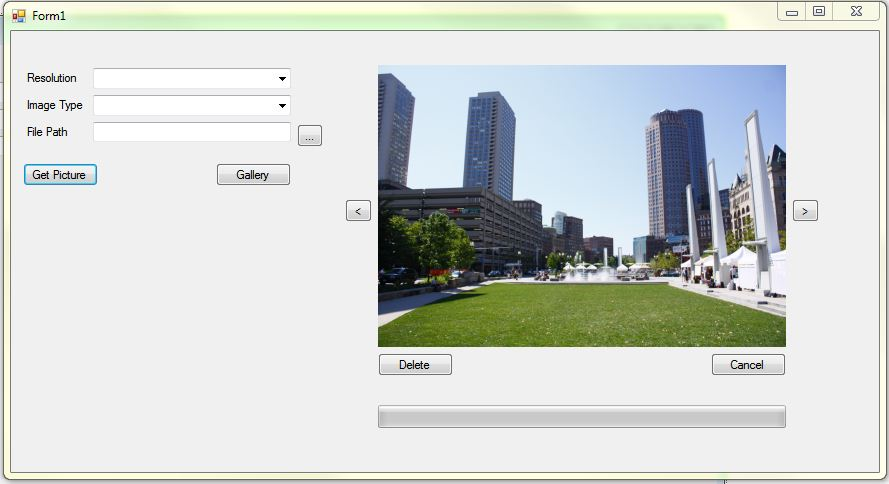
\includegraphics[scale=0.7]{figures/initialGUI.png} 
\end{center}
\caption{The initial design of GUI\label{ini_GUI}}
\end{figure}

\subsubsection{Initial Class Diagram}

Figure~\ref{ini_Class} shows initial design of classes to implement. The \texttt{JPEGFileReader} Class is use for decoding the JPEG file. The decoding method is in the plan of the final program because the image take a long time to download. So, if a  The method is that in the JPEG file, there are headers. In order to make the image progressively better, these header must be extracted. The method commandCheck use check each byte of the image for a \texttt{0XFF} value. For any JPEG file, 0XFF is the start of the header of the JPEG image. The huffman table and quantization table can transform from the byte value. 
\begin{center}
\begin{figure}[!hbtp]
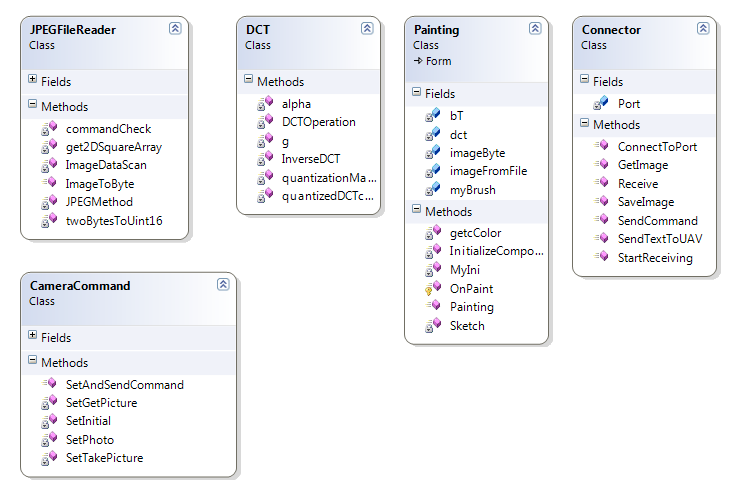
\includegraphics[width=150mm,height=100mm]{figures/initialClassDiagram.png} 
\caption{The initial design of GUI classes\label{ini_Class}}
\end{figure}
\end{center}
DCT has many math operation and equation which have to be implemented on the image viewer program. This include discrete cosine transform, and inverse discrete cosine transform. The inverse DCT for encoding:

\begin{equation}
f_{xy}=\sum_{u=0}^7\sum_{v=0}^7 \alpha(u) \alpha(v) F_{u,v} \cos\Big[\dfrac{\pi}{8}(x+\dfrac{1}{2})u\Big]\cos\Big[\dfrac{\pi}{8}(y+\dfrac{1}{2})v\Big]
\end{equation}

$x$ is the pixel row, for the integer $0< x< 8$

$y$ is the pixel column, for the integer $0< x< 8$

$\alpha(u)$ is a normalizing scale factor

$F_{u,v}$ is the reconstructed approximate coefficient at coordinates $(u,v)$
 
$f_{x,y}$ is the reconstructed pixel at coordinates $(x,y)$

This complicated function should implement in the ground station because if the picture is encoded in the compressed way, the ground station must be able to extract it. In the end, we have to determine whether is it faster to display image normally, or to do encoding/decoding JPEG file. The another downside of this method is that there are many encoding resource which work perfectly, but because of this is long and complex, it might cause some error and time consuming.
The painting class is supported by the DCT class. The intention of this class is to display an encoded image point by point on the picture box.By this method, the pictureBox can display an image at the first pixel.
The \texttt{CameraCommand} class design for send the data from the ground station to the camera. The idea is that make the camera sync with the payload by using the ground command. \texttt{SetAndSendCommand} use for set the byte command and then send it to the payload via the Console port. \texttt{SetGetPicture,SetInitial, SetPhoto, and SetTakePicture} methods are use for setting the correct byte in order to send the byte by using \texttt{SetAndSendCommand} class.

\subsubsection{Use Case Diagram}

Figure~\ref{GUI_useCase} shows a possible user action on the program. The user can save, open and delete any jpeg image from the computer. The program can also detect the corrupted image and ask the user to delete it. The user has an option to connect to the UAV. This is incase of the UAV is not connected properly. The most important function is get picture from the UAV camera. This will send and receive complex command which will be described. The internal program will process the byte and display the information as image onto the pictureBox. The user will then have an option to save the image and close the program.
\begin{figure}[!hbtp]
\begin{center}
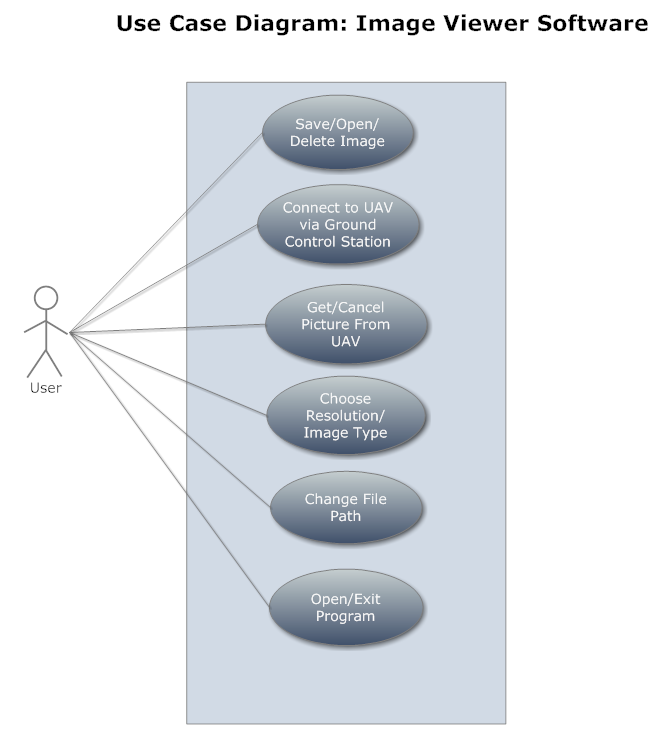
\includegraphics[scale=0.6]{figures/userCase.png} 
\end{center}
\caption{Use case diagram of the GUI\label{GUI_useCase}}
\end{figure}



\subsection{Approach: Different C\# .NET Classes}
The C\# language on Microsoft Visual Basic Studio is a development environment for creating our Ground Station Image Viewer application. Choosing the right class to connect to the port helps the developer save time to program the application. The class should be able to connect to the UAV port and it must be able to send both byte and string command and receive bytes camera data from the UAV.  The C\# program has two .NET classes that can connect to port. They are SerialPort Class and Socket Class. 
\subsubsection{SerialPort Class}
The System.IO.Ports namespace contains classes for controlling serial ports. The SerialPort class is the most important one.It has ability to synchronous and event-driven I/O, access to pin and break states, and access to serial driver properties\cite{peak_netFrame}. It can change the port properties such as the stop bit, parity bit, baud rate, etc. It has handshake function that communicate to the port and report if the data or token was received successfully.
By using this class, the COM port setting has to be memorized which will be simple to load and saves from/to disk.In the process both public and private fields of the object and the name are converted to a stream of bytes.

\begin{lstlisting}[caption=Serial Port class connection\, read and write method, label=serialPortconn]
SerialPort( portName, baudRate, parity bit, dataBits, StopBits ) 
SerialPort.Read(Char(),Int32,Int32);
SerialPort.Write(Char(), Int32, Int32)	;
\end{lstlisting}

The advantage of using this class is that the port can change baud rate, handshaking, parity bit, and stop bit. It has an ability to change the internal structure of signal of hardware. The class has a read and writes methods which connection with TCP/IP is possible.
However, the implementation of the class has many unnecessary set up and the code will be very long and can cause error, and it is not possible to reprogram the UAV.
Write() is a SerialPort's public method is use to send data of bytes to an output buffer at the specified offset, it writes a specified number of characters to the serial port using data from a buffer.
Reads method read a number of bytes from the SerialPort input buffer and writes those bytes into a byte array at the specified offset.

If the UAV baud rate is different from the program baud rate, the error will occur.
The parity bit, and end bit and baud rate have to be set up in order to connect to the port, but these set up in UAV already.
\subsubsection{Socket Class}
The Socket is more programmer friendly, robust and a high level connection class. The socket class is use to send and receive data, in similar method as an open file allows an application to read and write data to stable storage.  It also makes a simple handshaking between the client and server machines. It can connect to multi clients, which this is necessary for a multi-port which we are using. The program can easily connect to the port by using the method in Listing\ref{socketClasscrs} .
This method takes the baud rate and parity bit configuration from the UAV so the setup is the same. This class sends and array of bytes to the console port and to the data stream port and receive data from the port by code in Listing\ref{socketClasscrs}.

\begin{lstlisting}[caption=Socket class connect receive and send method,label=socketClasscrs]
Connect (String host name,Int32 port number)
Send(byte[] command, Int32 length, SocketFlags)
Receive(byte[] data, Int32 length, SocketFlags)
\end{lstlisting}